\chapter{Conception et Développement de la Plateforme} \label{chap:implementation}

\section{Présentation Générale du Projet}

Dans le cadre de ce projet, nous avons développé une plateforme web interactive dédiée au \textbf{pricing d'options européennes}, permettant de comparer différentes méthodes de valorisation sur des données réelles du marché. L'application est accessible à l'adresse suivante :

\begin{center} \url{https://options-price.vercel.app/} \end{center}

Le projet repose sur une architecture \textbf{full-stack moderne} :

\begin{itemize} \item \textbf{Frontend} : développé en \textbf{Next.js}, un framework React, et déployé sur \textbf{Vercel}. \item \textbf{Backend} : construit avec \textbf{FastAPI}, framework Python pour des APIs rapides, hébergé sur un serveur dédié. \item \textbf{Dépôt GitHub du projet} : \begin{center} \url{https://github.com/hassanelq/Options-pricing} \end{center} \end{itemize}

La plateforme propose notamment : la sélection de modèles de pricing, la récupération automatique de données de marché, la calibration de modèles stochastiques, et la visualisation intuitive des résultats.

\section{Architecture du Projet}

Le projet est organisé en deux principales parties :

\begin{itemize} \item \textbf{Client (Frontend)} : situé dans \texttt{client/}, développé sous \texttt{Next.js}. \item \textbf{Server (Backend)} : situé dans \texttt{server/}, développé sous \texttt{FastAPI}. \end{itemize}

\subsection*{Client (Next.js)}

\begin{itemize} \item \texttt{app/Components} : composants de l'interface utilisateur. \item \texttt{app/Options-pricing} : logique métier liée au pricing d'options. \item \texttt{app/methodology} et \texttt{app/documentation} : contenu méthodologique et explicatif. \end{itemize}

\subsection*{Server (FastAPI)}

\begin{itemize} \item \texttt{models/} : implémentation des modèles Black-Scholes et Heston. \item \texttt{utils/} : modules utilitaires de calibration, de fetching des données, et tests. \item \texttt{routes/} : définition des API REST. \item \texttt{main.py} : point d'entrée principal. \end{itemize}

\section{Parcours Utilisateur et Fonctionnalités Clés}

\subsection{Configuration de l'Option}

L'utilisateur commence par configurer les paramètres de base :

\begin{itemize} \item Style de l'option (européenne uniquement), \item Modèle de pricing (Black-Scholes ou Heston), \item Type d'actif (ETFs, indices, actions). \end{itemize}

\begin{figure}[H] \centering 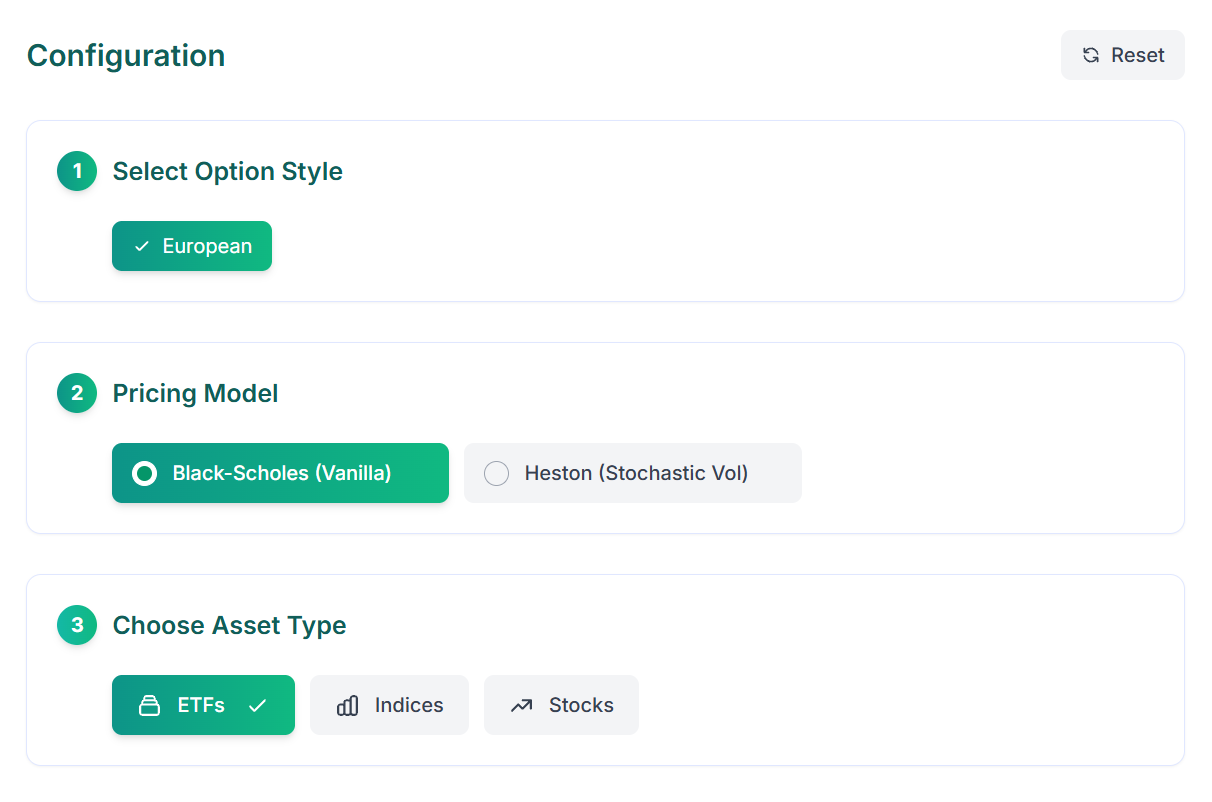
\includegraphics[width=0.9\textwidth]{images/1.png} \caption{Configuration de l'option : style, modèle, et type d'actif} \end{figure}

\subsection{Recherche et Chargement des Données de Marché}

L'utilisateur recherche un actif (par ex., \texttt{SPY}) et importe les données d'options disponibles en temps réel :

\begin{figure}[H] \centering 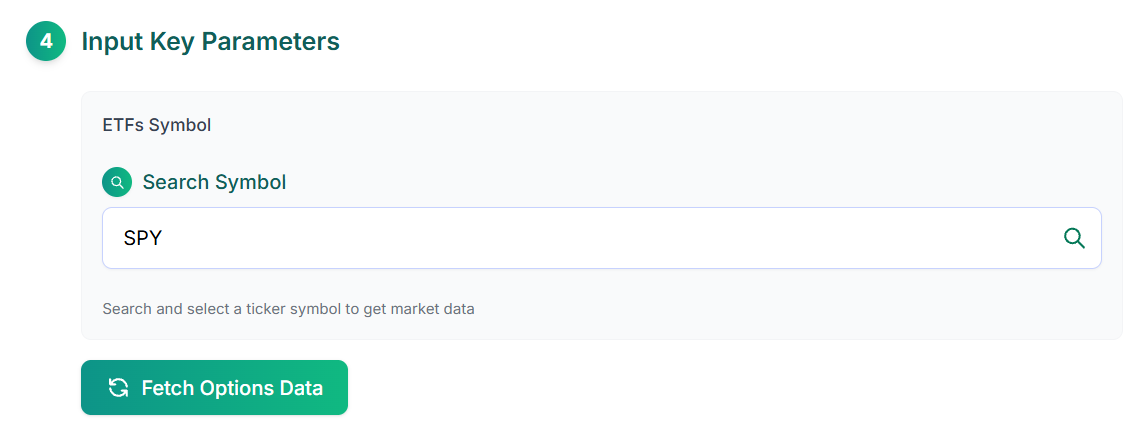
\includegraphics[width=0.9\textwidth]{images/2.png} \caption{Recherche du symbole et importation des données} \end{figure}

\subsection{Sélection d'un Contrat d'Option}

Une liste d'options est affichée (calls et puts) avec les strikes, prix, volatilités implicites, volumes et échéances. L'utilisateur peut sélectionner un contrat spécifique via un bouton \texttt{Auto-Fill}.

\begin{figure}[H] \centering 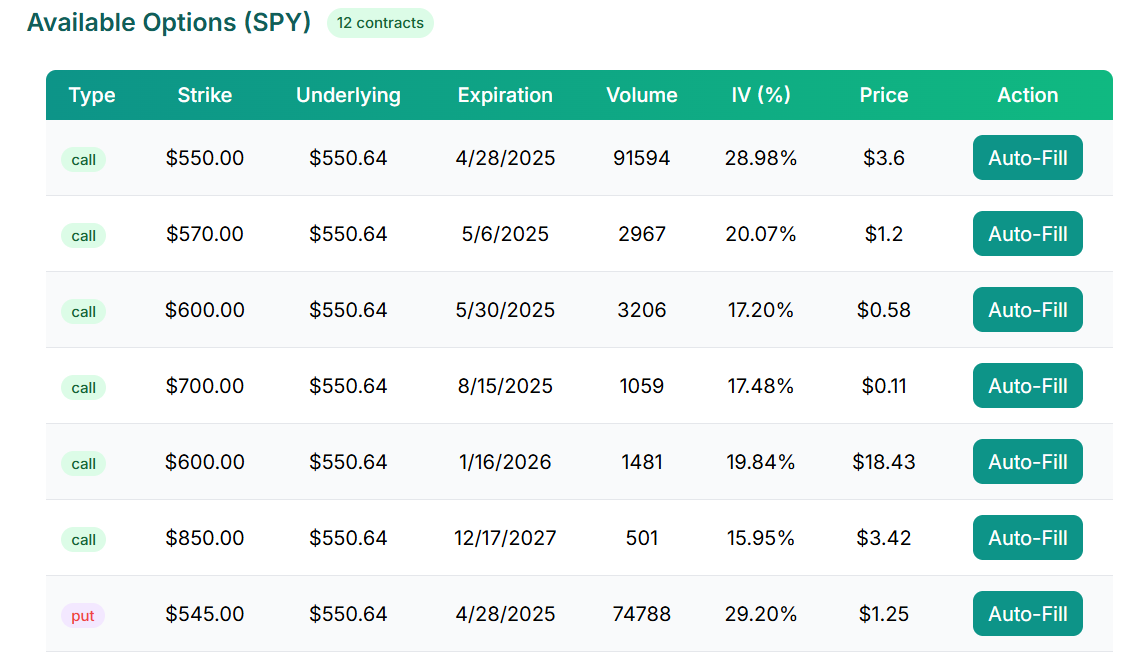
\includegraphics[width=0.9\textwidth]{images/3.png} \caption{Liste d'options disponibles pour l'actif sélectionné} \end{figure}

\subsection{Remplissage Automatique des Paramètres}

Après sélection, les informations critiques sont automatiquement remplies : strike, spot, volatilité implicite, temps jusqu'à maturité, taux sans risque.

\begin{figure}[H] \centering 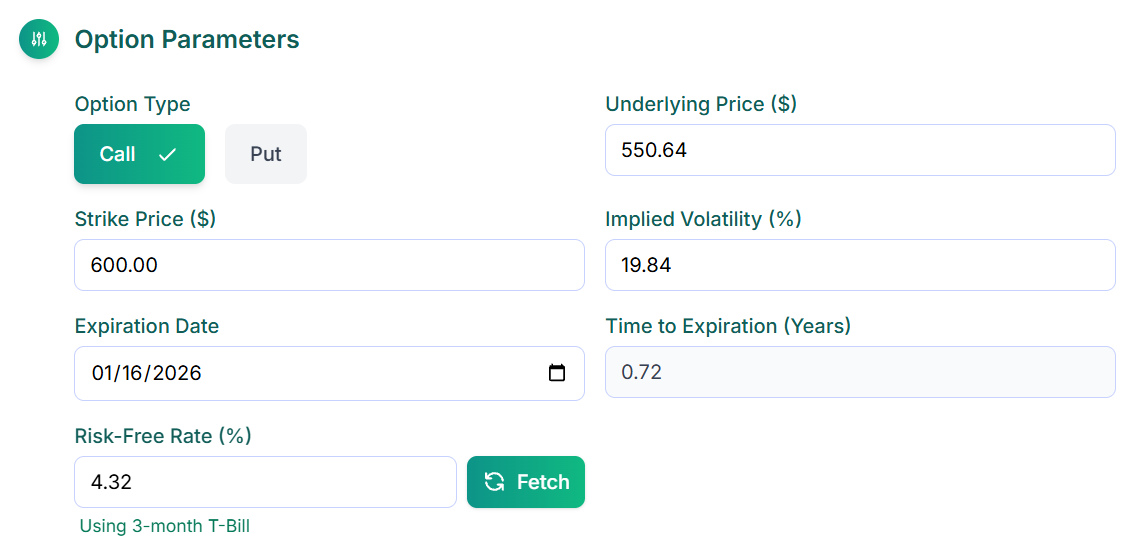
\includegraphics[width=0.9\textwidth]{images/4.png} \caption{Pré-remplissage des paramètres de l'option sélectionnée} \end{figure}

\subsection{Choix de la Méthode de Pricing et Paramétrage du Modèle de Heston}

Pour le modèle de Heston, les utilisateurs peuvent :

\begin{itemize} \item Soit saisir manuellement les paramètres ($\kappa$, $\theta$, $\sigma$, $\rho$, $v_0$), \item Soit lancer une \textbf{calibration automatique} en cliquant sur \texttt{Calibrate Parameters}. \end{itemize}

Deux méthodes de pricing sont proposées : \begin{itemize} \item Solution semi-analytique par transformée de Fourier, \item Simulation Monte Carlo pour payoffs plus complexes. \end{itemize}

\begin{figure}[H] \centering 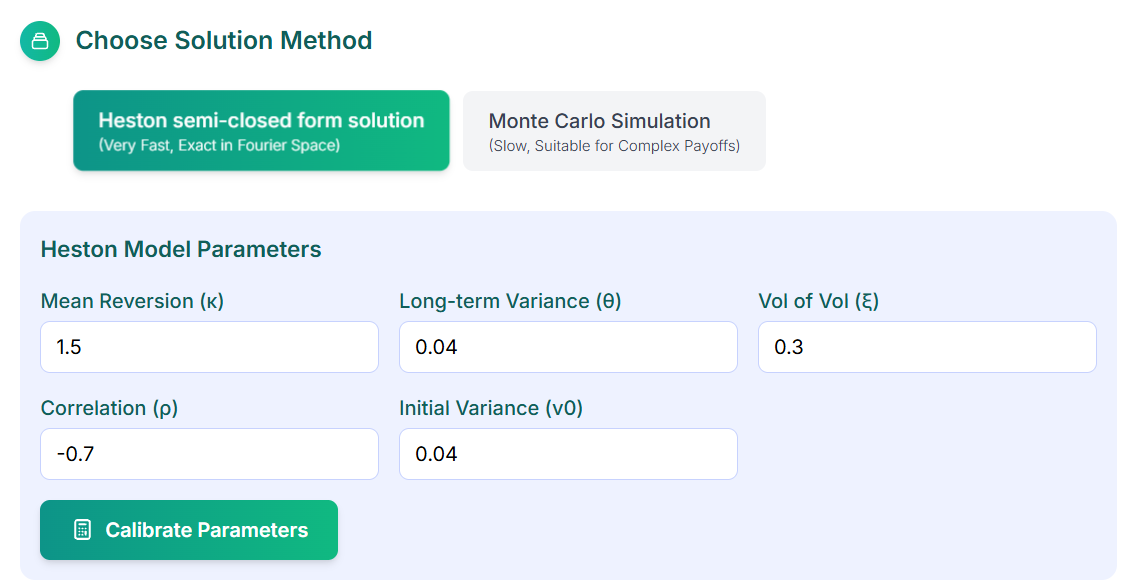
\includegraphics[width=0.9\textwidth]{images/5.png} \caption{Saisie manuelle ou calibration automatique des paramètres du modèle de Heston} \end{figure}

\section{Affichage des Résultats}

\subsection{Résumé des Paramètres}

Un tableau récapitule tous les paramètres saisis ou calibrés : prix spot, strike, volatilité, taux sans risque, méthode de solution, type d'option, etc.

\begin{figure}[H] \centering 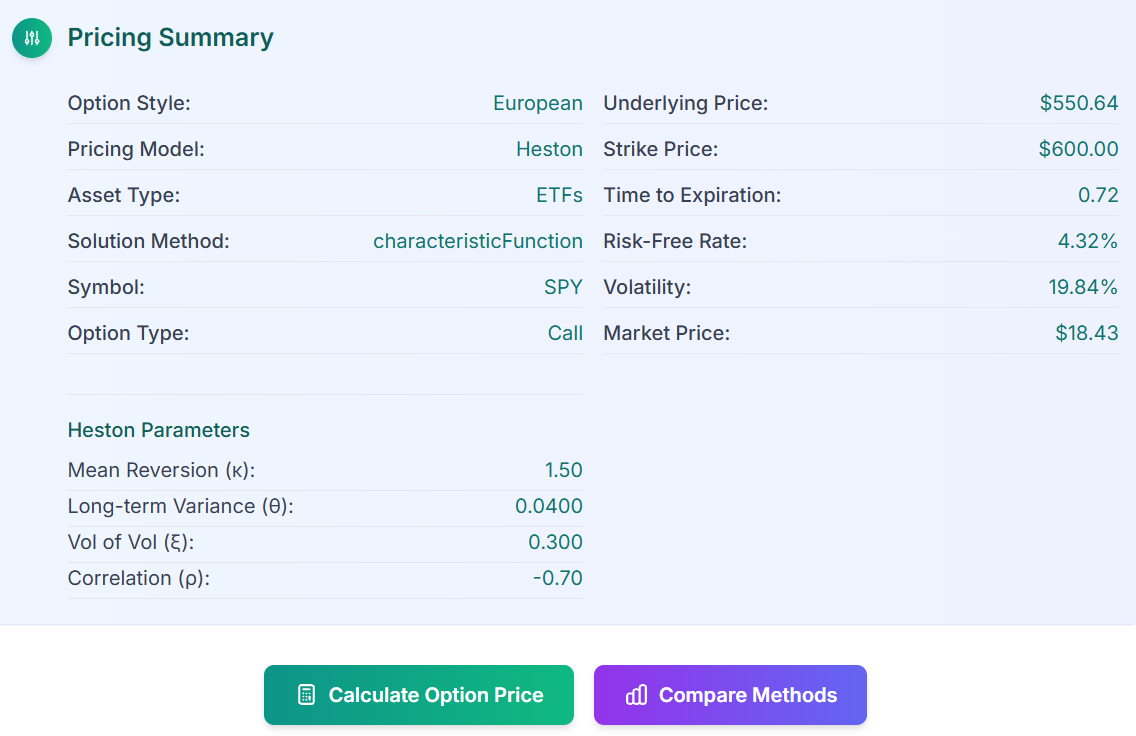
\includegraphics[width=0.9\textwidth]{images/6.png} \caption{Résumé des paramètres d'entrée pour le pricing} \end{figure}

\subsection{Résultats du Pricing}

Le prix de l'option est affiché ainsi que l'écart relatif par rapport au prix de marché, accompagné du temps de calcul.

\begin{figure}[H] \centering 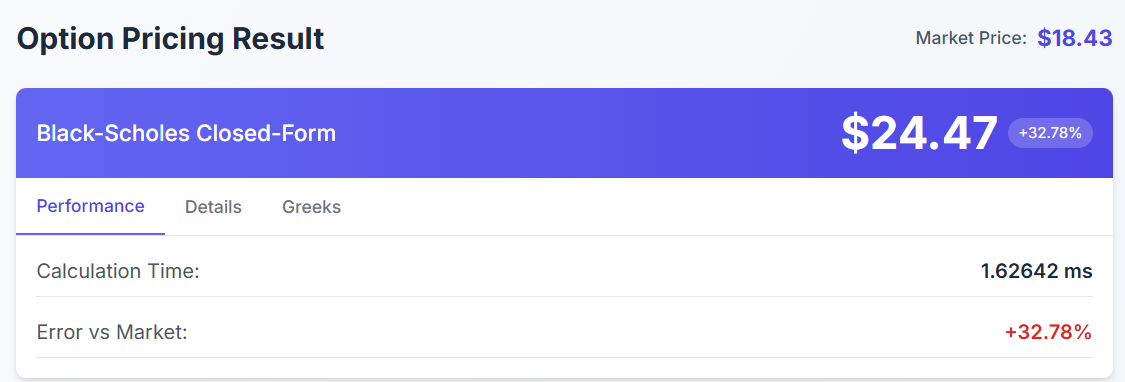
\includegraphics[width=0.9\textwidth]{images/7.png} \caption{Résultat du pricing (prix, temps de calcul, erreur)} \end{figure}

\subsection{Visualisation du Payoff et du Profit}

Deux diagrammes sont générés automatiquement pour représenter :

\begin{itemize} \item Le payoff et le profit du call acheté (\texttt{Long Call}), \item Le payoff et le profit du call vendu (\texttt{Short Call}). \end{itemize}

\begin{figure}[H] \centering 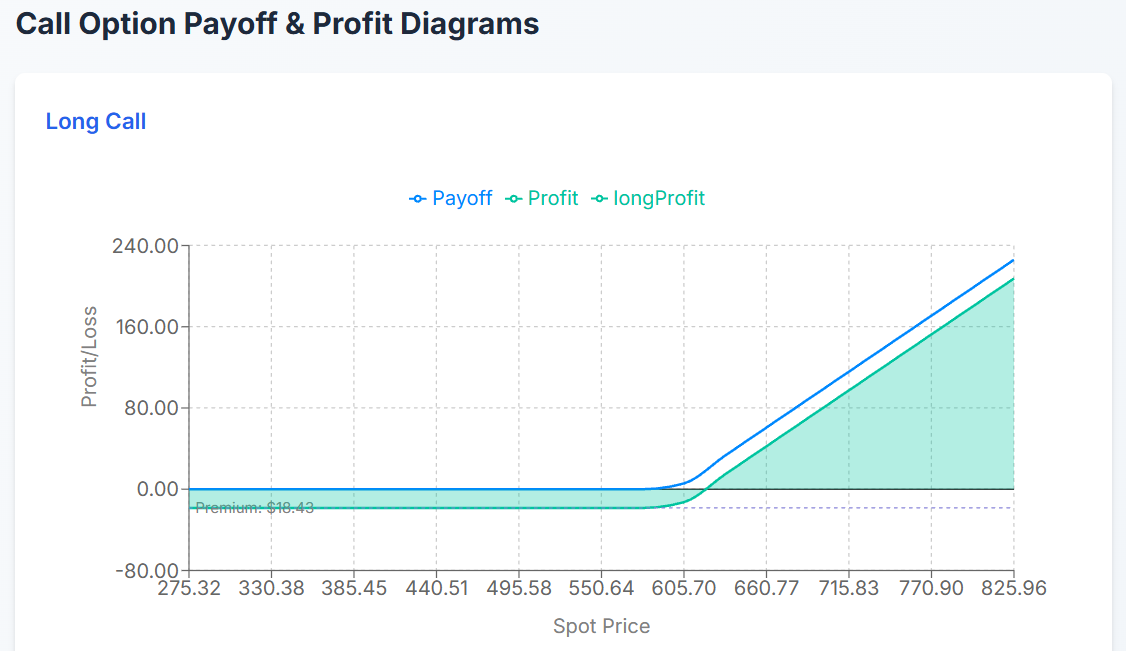
\includegraphics[width=0.9\textwidth]{images/8.png} \caption{Diagramme de profit pour un long call} \end{figure}

\begin{figure}[H] \centering 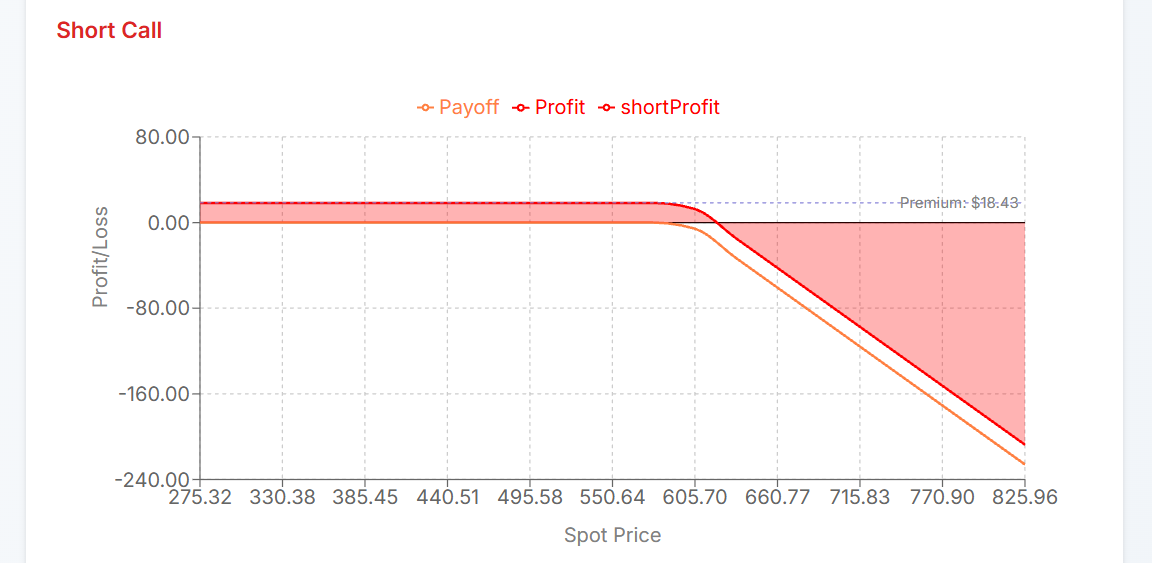
\includegraphics[width=0.9\textwidth]{images/9.png} \caption{Diagramme de profit pour un short call} \end{figure}

\section{Conclusion}

La plateforme développée fournit une solution complète, rapide et intuitive pour l'analyse du prix d'options européennes en utilisant à la fois des modèles classiques (Black-Scholes) et avancés (Heston). En combinant les dernières technologies web (Next.js, FastAPI) avec des méthodes quantitatives de pointe, elle offre une expérience utilisateur fluide tout en restant rigoureuse sur le plan financier.